\documentclass{article}
\newcommand{\Mhalo}{\ensuremath{M_{\rm halo}}}
\newcommand{\MhaloPeak}{\ensuremath{M_{\rm halo, peak}}}
\newcommand{\vmp}{\ensuremath{V_{\rm max}@M_{\rm peak}}}
\newcommand{\tlogten}{{\rm log}_{10}}
\newcommand{\Mstar}{\ensuremath{M_{\ast}}}
\newcommand{\M}[1]{\ensuremath{M_{\ast,\,\rm #1}}}
\newcommand{\eg}{{\it e.g.\/}}


\usepackage{graphicx}
\usepackage{amsmath}
\usepackage{hyperref}



\begin{document}

\section{Introduction}

We want to make a convincing mock. To do this, we will take an N-body sim (the 1Gpc MDPL) and put galaxies in it using the~\cite{Behroozi2010} prescription.

\begin{equation}
    \label{eq:sm_hm_functional_form}
    \tlogten{}(\Mhalo{}) = \tlogten{}(M_1) + \beta~\tlogten{}(\frac{\Mstar{}}{\M{0}}) + \frac{(\frac{\Mstar{}}{\M{0}})^{\delta}}{1 + (\frac{\Mstar{}}{\M{0}})^{- \gamma}} - \frac{1}{2}
\end{equation}


We also add a mass varying scatter
\begin{equation}
\sigma = a \Mhalo + b
\end{equation}

From \cite{Leauthaud2012} we know the parameters for the functional form are approximately $10^{12.52}, 10^{10.91}, 0.45, 0.6, 1.83$ and from my paper we know that the scatter is approximately $0.3$ and $0.18$ at $\Mhalo{} = 10^{13}$ and $10^{15}$.

However, we want to make sure that the mock matches HSC as closely as possible. We will therefore optimize these parameters to fit the SMF and clustering, beginning from these starting points.

\section{Optimizing model}

\subsection{\Mhalo{} vs \vmp{}}

Initially we modelled (as in the previous equation) \Mstar{} as a function of \Mhalo{} and \MhaloPeak{}. However, per Peter we should instead be using \vmp{}. I think this is because \Mhalo{} begins to be stripped before a halo merger takes place, while \vmp{} continues to increase (or at least stays constant). This causes a problem as we now need a functional form to relate $\Mstar(\vmp{})$

\begin{figure}[h]
    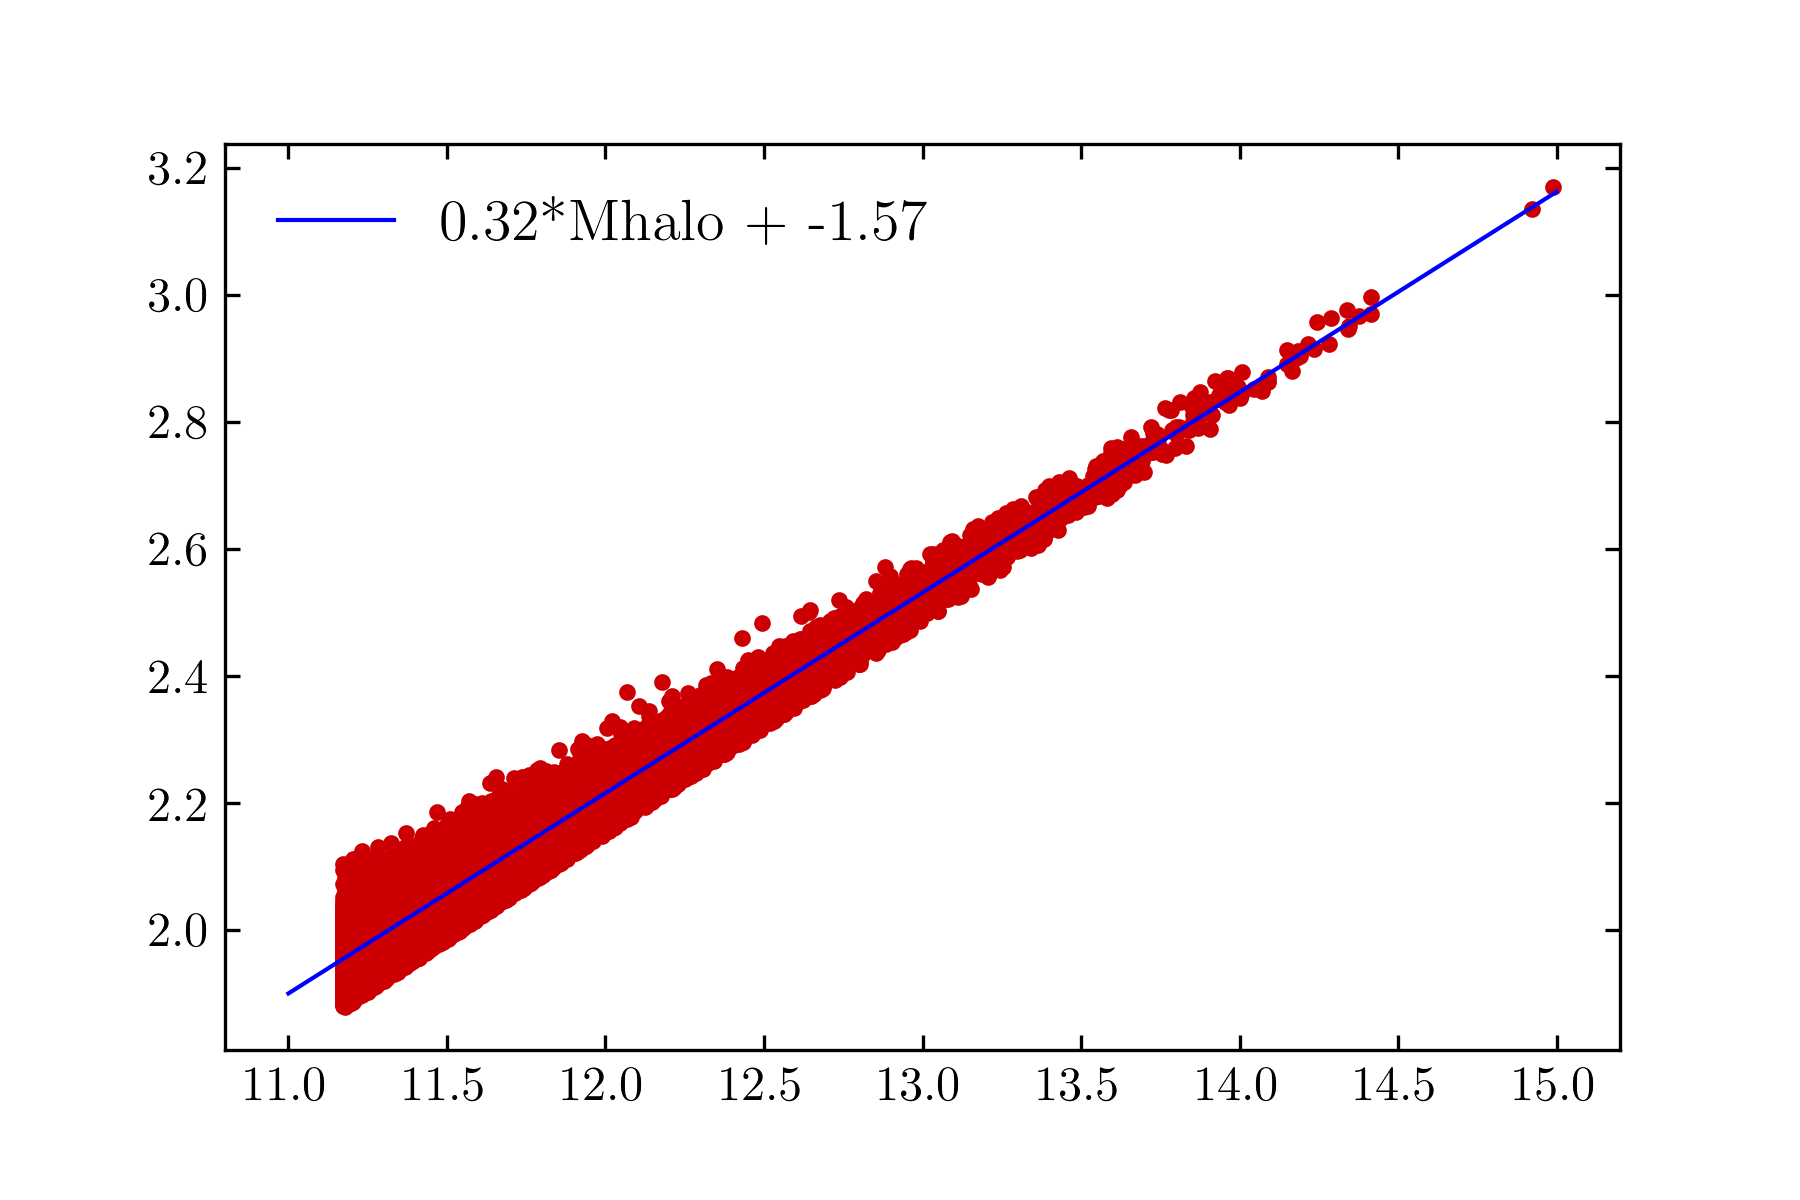
\includegraphics[width=\textwidth]{images/mhalo_vs_vmax.png}
    \caption{
        \vmp{} -- \Mhalo{} relation.
        \label{fig:mhalo_vs_vmax}
    }
\end{figure}

\autoref{fig:mhalo_vs_vmax} shows the relation between \vmp{} and \Mhalo{}. This is roughly linear in log space, so we can write:

\begin{equation}
    \begin{aligned}
        &\tlogten{}(\vmp{}) = m\ \tlogten{}(\Mhalo{}) + c \\
        &\tlogten{}(\vmp{}) = m * (\tlogten{}(M_1) + \beta~\tlogten{}(\frac{\Mstar{}}{\M{0}}) + \frac{(\frac{\Mstar{}}{\M{0}})^{\delta}}{1 + (\frac{\Mstar{}}{\M{0}})^{- \gamma}} - \frac{1}{2}) + c\\
    \end{aligned}
\end{equation}

We now have two options:
1) Use this new function with the known $m$ and $c$ and the old starting parameters
2) Numerically find (guess) a new starting point for the five numbers that folds $m$ and $c$ into them. I did this.

This is not purely guessing. We can rationalise that $M_1$ will decrease significantly (as $\vmp{} < \Mhalo{}$), $\M{0}$ will stay the same as the kink will be in about the same place. We can then guess at $\beta, \delta, \gamma$. We plot a couple of guesses at this and get the params of: $10^{2.4}, 10^{10.91}, 0.45, 0.3, 0.2$. We can use \autoref{fig:mhalo_vs_vmax} to map the scatter params. We parameterize this as a slope and a y intercept. In mass space this would be $-0.06, 1.08$. In velocity space it is approximately $-0.1, 0.5$.

We also note that \autoref{eq:sm_hm_functional_form} relates $\Mhalo(\Mstar)$, or $\vmp(\Mstar)$. We numerically invert this to get the inverse.

\subsection{HaloTools?}

Halotools is awesome and we should use it as much as possible. It also has a number of functions for creating a \cite{Behroozi2010} model. This seems great!

However, I didn't know about this when I started working on it and the actual part of the my code that halotools would take the part of is tiny. It is just the mapping of \vmp{} to \Mstar{}.
I have compared to ensure that my code and halotools are identical. The only difference is that my code assumes that all parameters (\eg{} $M_1$) have no little h. While in halotools they are assumed to have littleh of 0.7. Both will work fine they will just give different values for the same numerical values.

\subsection{Comparisons to observations}

We have an HSC galaxy catalog and an HSC SMF. Using the galaxy catalog we construct an estimate of clustering the 'counts in cylinders'.
For this we define a cylinder 1Mpc in radius and 10Mpc in half length. We then pick a mass cut, \eg{} $10^{11}$.
Around each galaxy larger than the mass cut we count the number of galaxies between the mass cut and $0.1$ dex below it.
From this we construct a clustering signal using the Landay Szaly estimator using a random catalog.

We do this for a number of mass cuts.


\subsection{Optimization}
Given a halo catalog (MDPL) and a way to add galaxies to them (see previous 2 sections) we can now generate a mock. Each time we generate a mock we compute an SMF and an 'counts in cylinders' clustering signal analagous to what we have in data. We want the SMF and the clustering to be similar to the data.

To optimize this we assume that all points are uncorrelated and try to minimize error, scaled by the uncertainties on each point.

Note that we don't use MCMC to optimize as that is not what it is good at \cite{Hogg2018}. It is slow and also a bad optimizer for high dimensional problems \cite{Betancourt2017}. A downside of this though is that we don't get uncertainty estimates and so we don't know if some other parameter set is just a bit worse than the bestfit or is terrible. If we need that I can run an MCMC.

After running this, the best fit model has params: \\$2.379, 10.92,  0.356,  0.185,  0.278, -0.110, 0.519$

This fits the SMF and clustering well (see \autoref{fig:fit_smf}, \autoref{fig:fit_clust}).

\begin{figure}[h]
    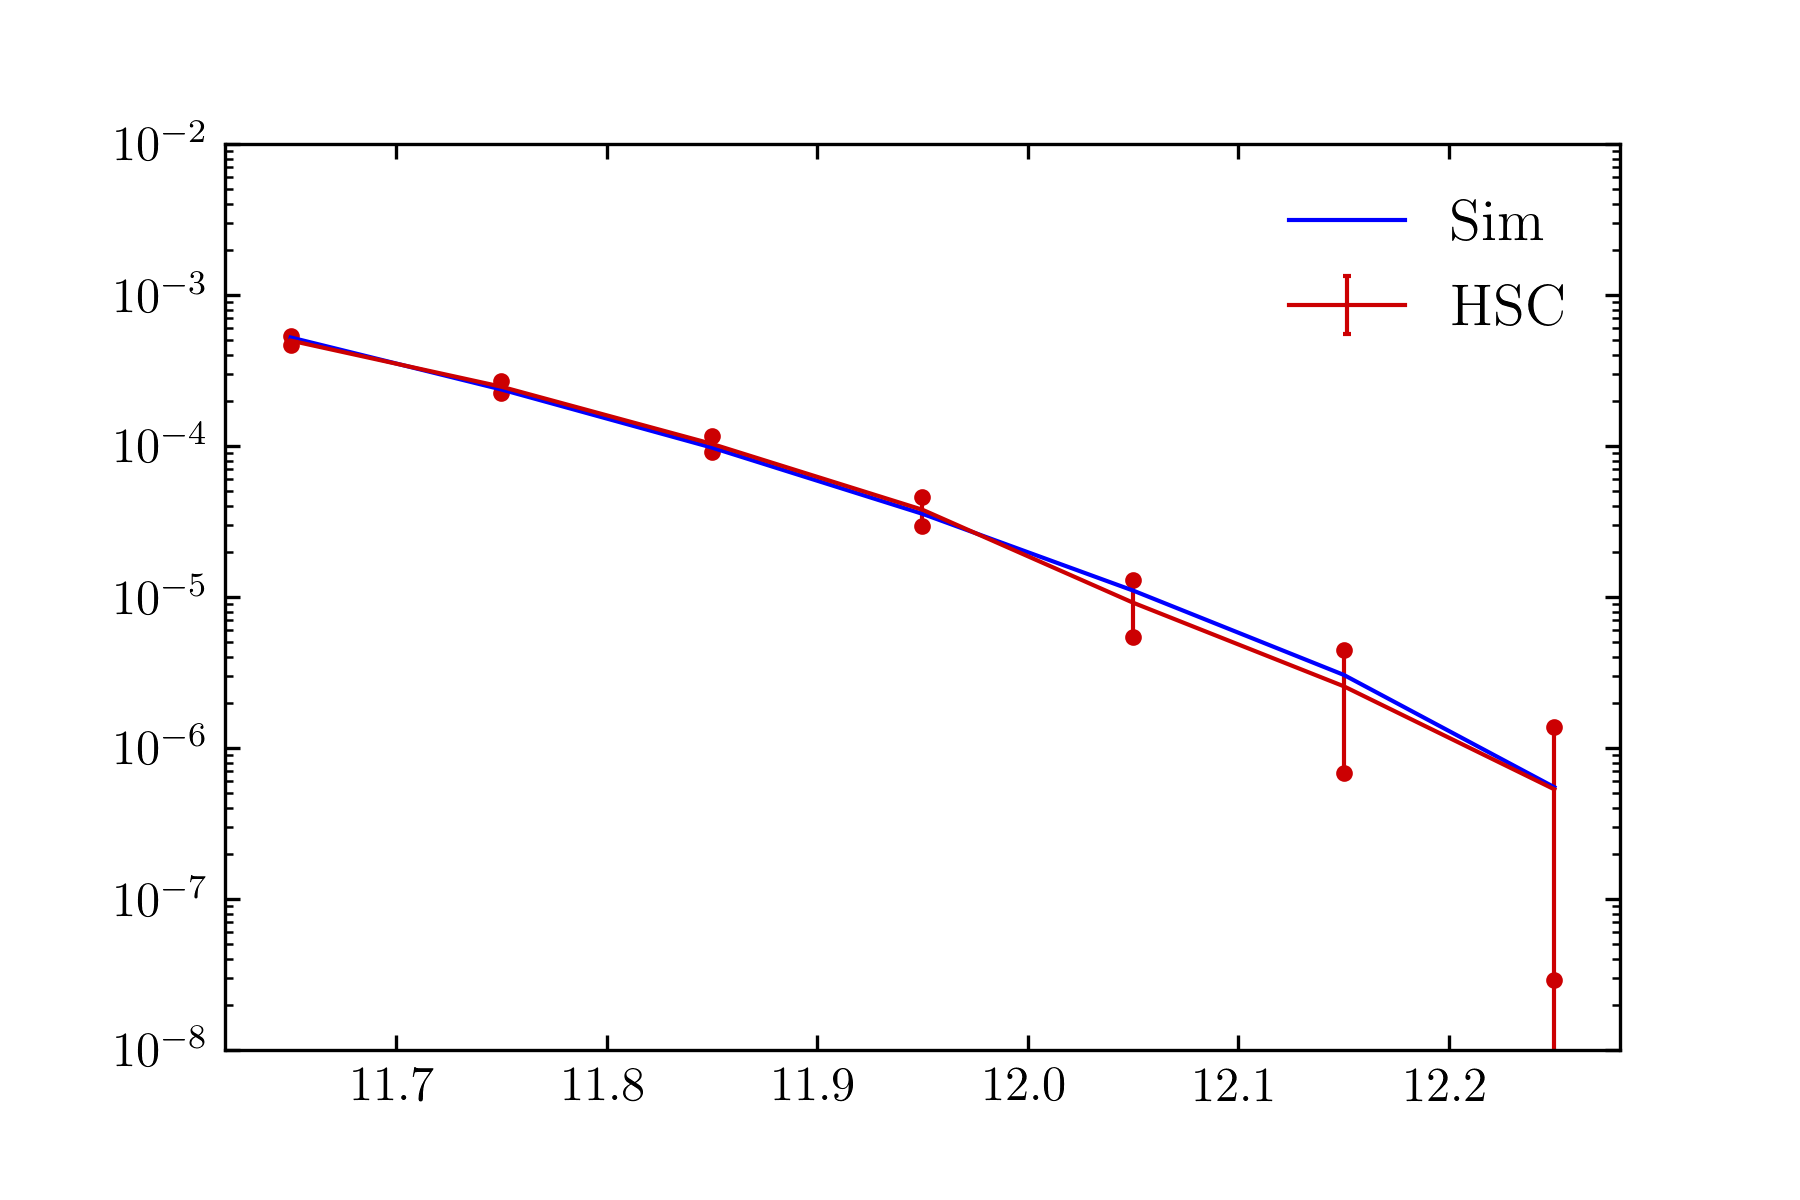
\includegraphics[width=\textwidth]{images/fit_smf.png}
    \caption{Fit to SMF - pretty good
        \label{fig:fit_smf}
    }
\end{figure}

\begin{figure}[h]
    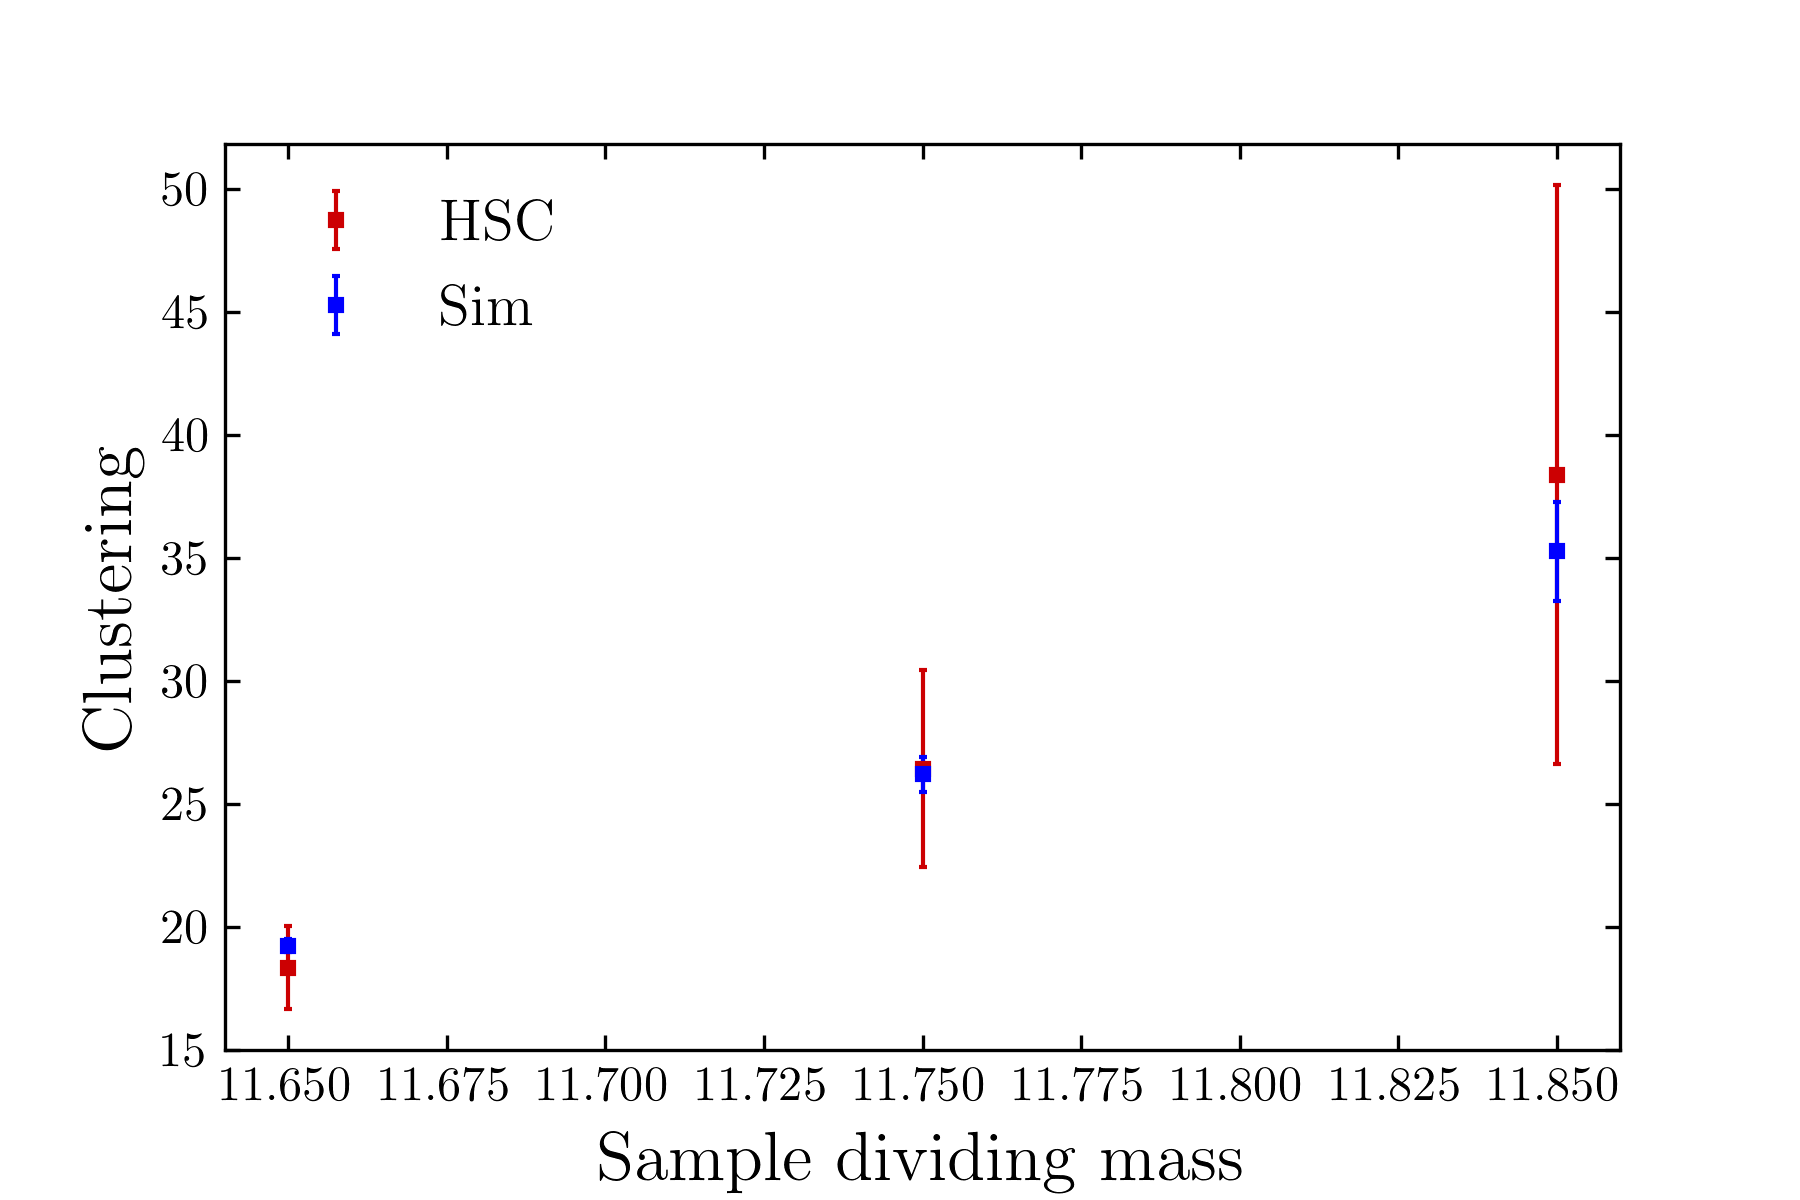
\includegraphics[width=\textwidth]{images/fit_clust.png}
    \caption{Fit to clustering - pretty good
    \label{fig:fit_clust}
    }
\end{figure}

\section{Tests}

While we have shown that the functional form is flexible enough to fit the HSC SMF and clustering, this doesn't mean that the resulting mock is a good model. It might have got a bunch of other important things that we didn't fit for wildly wrong. Let's check a couple of those things, and also just sanity check the mock.


\subsection{Scatter}
Based on how we parameterize scatter (linear decrease vs \vmp{}), we expect for it to linearly decrease with increasing \Mhalo{}. We also expect it to roughly match the numbers we found in the UM. It does -- see \autoref{fig:scatter}.

\begin{figure}[h]
    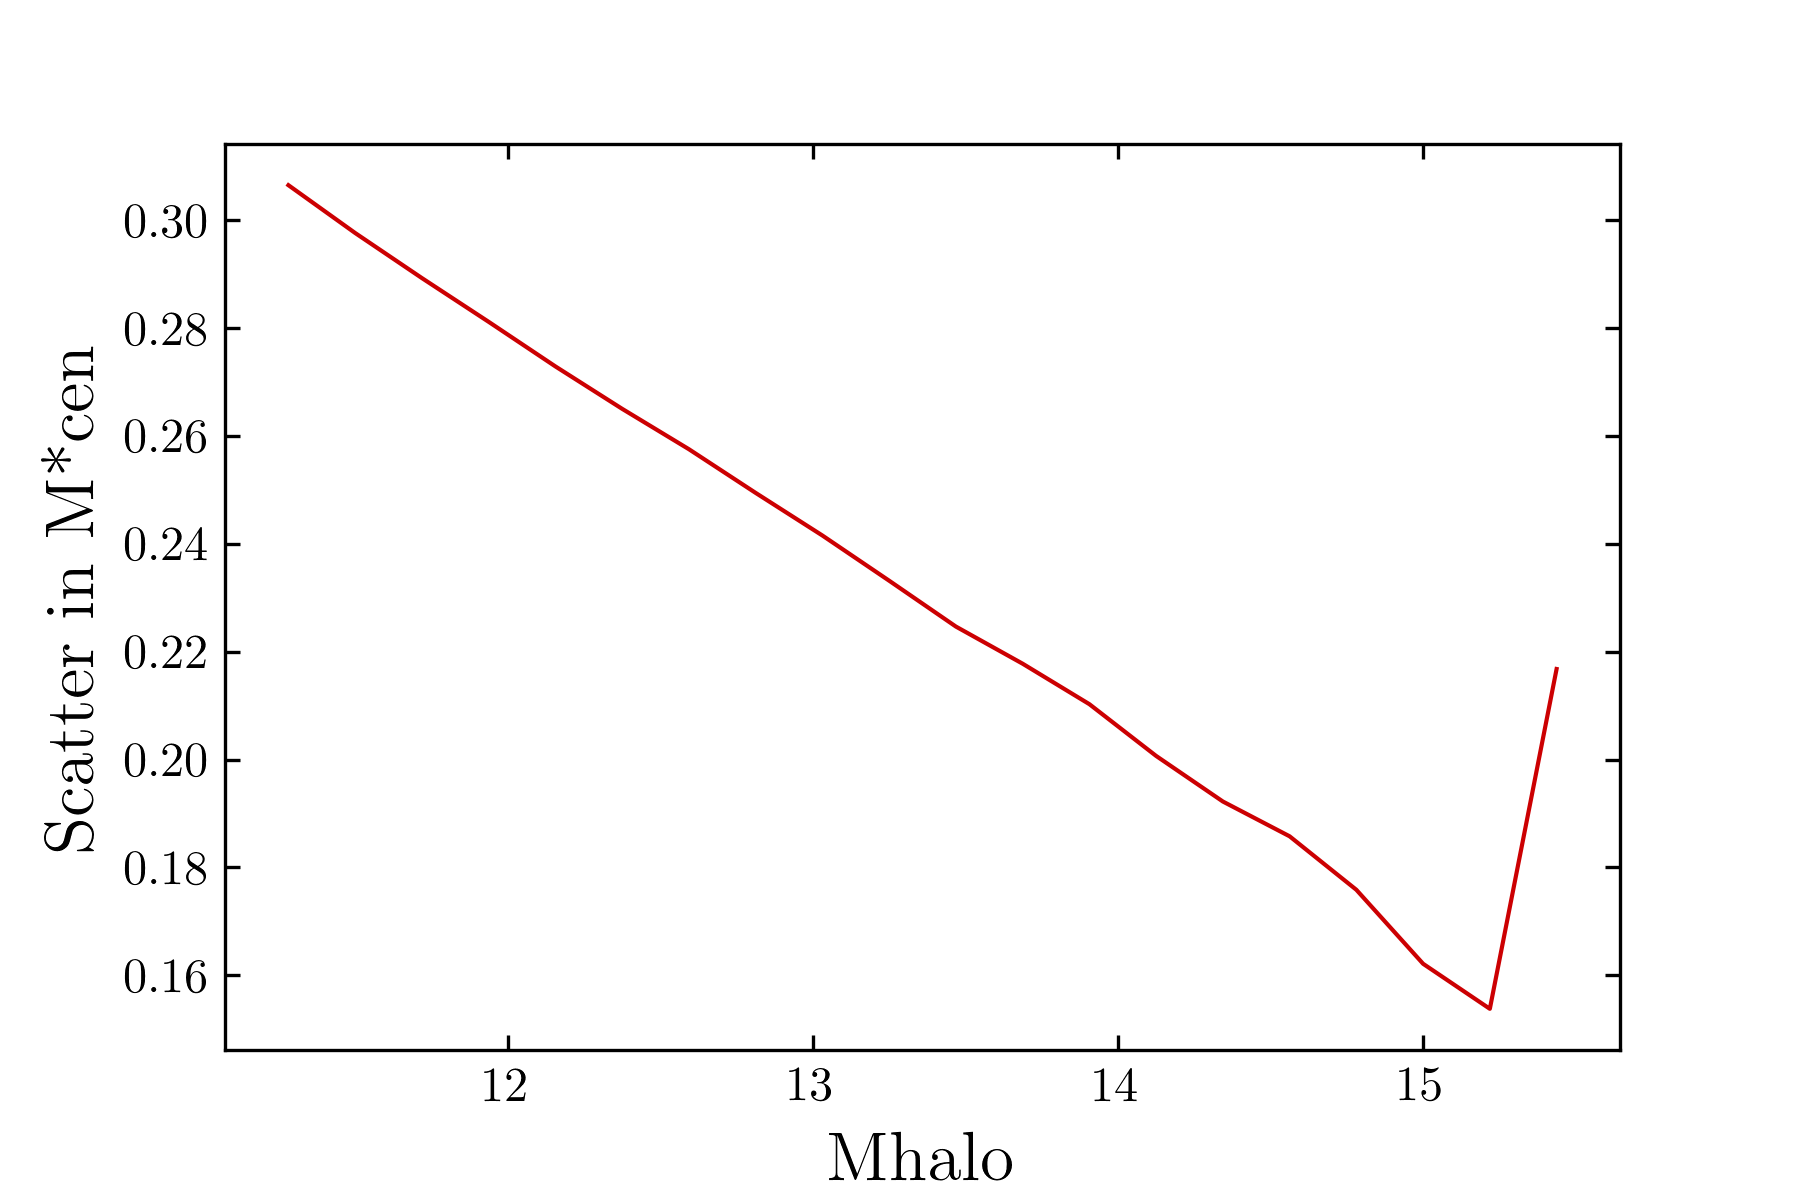
\includegraphics[width=\textwidth]{images/scatter_mcen_mhalo.png}
    \caption{Looks like what we expect from the scatter params. Ignore the kick up at the end, I'm pretty sure the uncertainty on that point is huge.
    \label{fig:scatter}
}
\end{figure}


\subsection{Two point correlation function}

Does our two point autocorrelation function look good? Compare to \cite{Tinker2017} who used CMASS. See \autoref{fig:2pcf}.

\begin{figure}[h]
    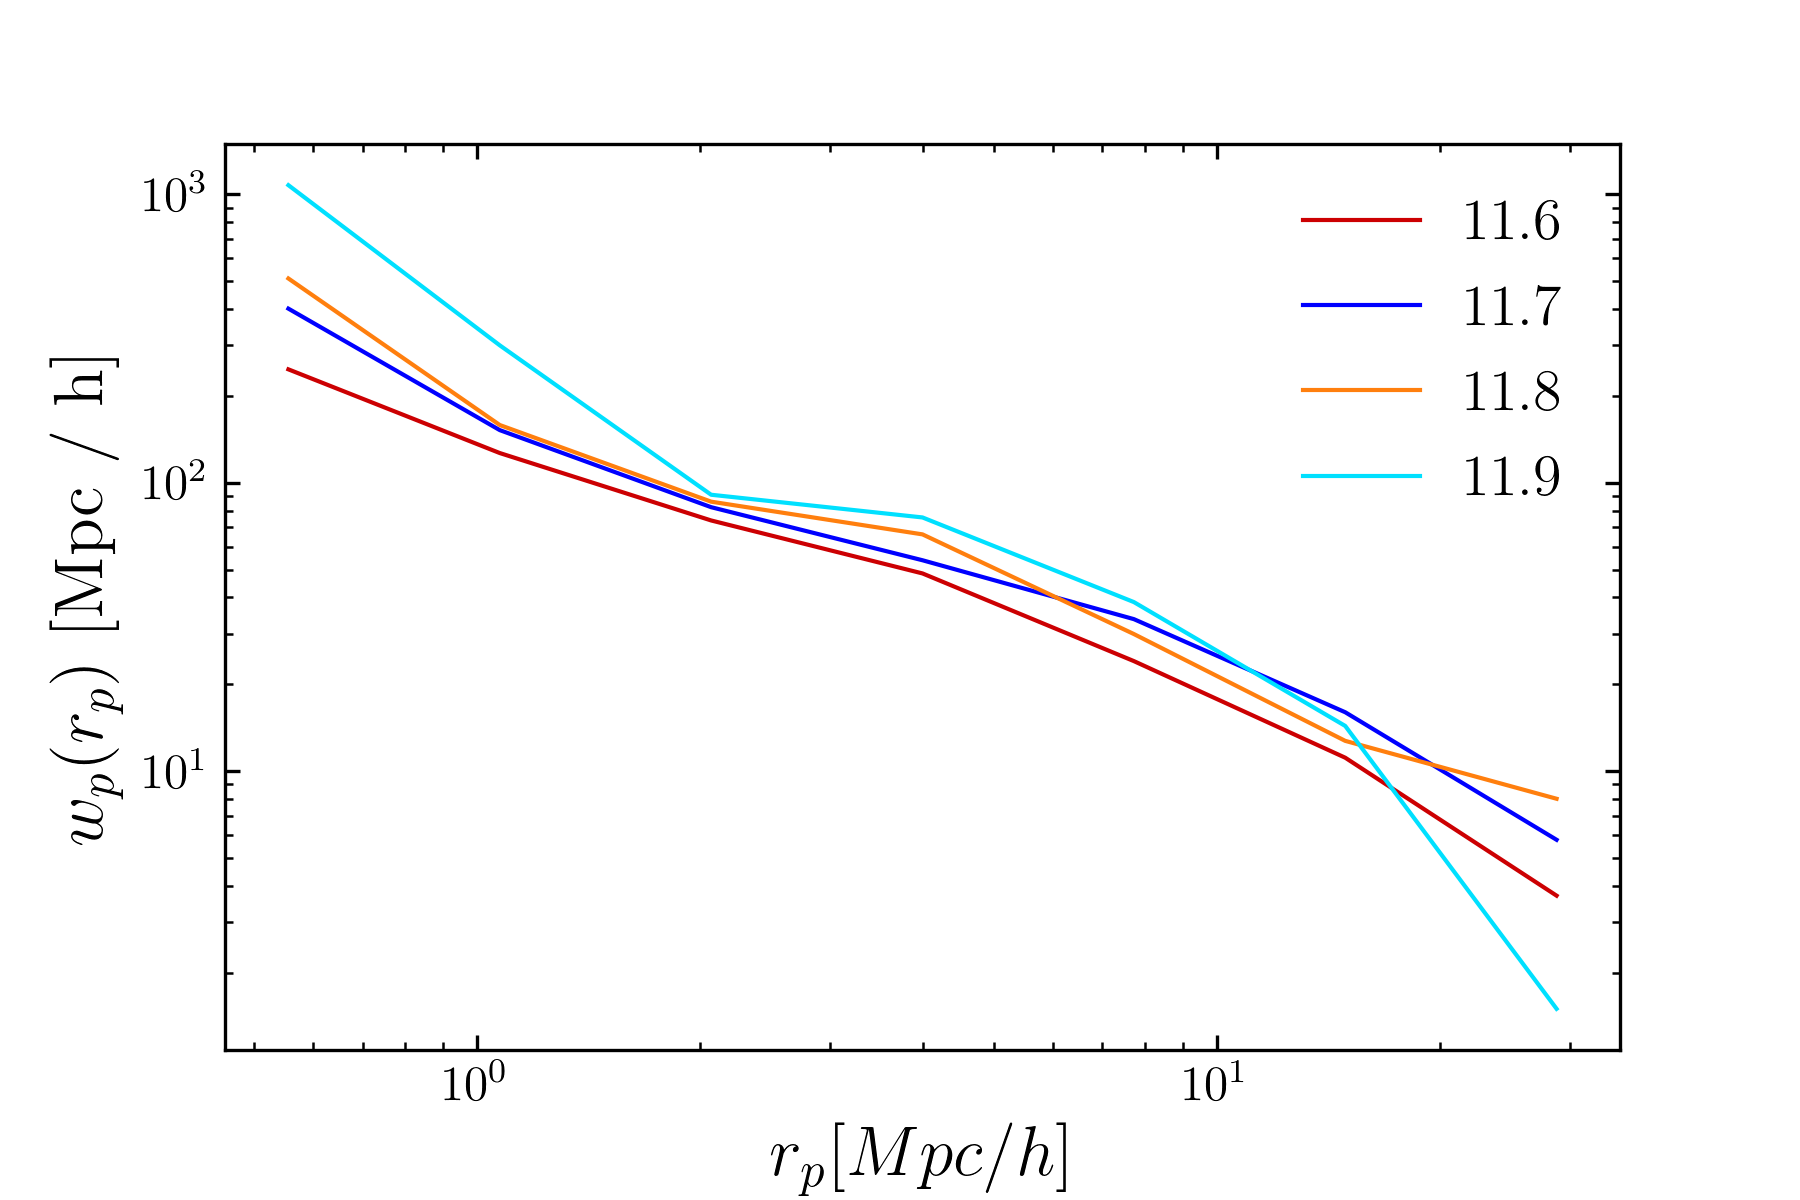
\includegraphics[width=\textwidth]{images/2pcf.png}
    \caption{Satellite fraction with 2 methods of cluster finding. The first just uses Rockstar cen/sat. The second constructs cylinders 1MPC in radius and 10MPc half length. A galaxy is a satellite if it is in the cylinder of a larger galaxy. The mock matches HSC well.
        I'm not sure how surprised we should be about this as it seems to follow pretty directly from clustering?
    \label{fig:2pcf}
}
\end{figure}

\subsection{Satellite Fraction}

We want the fraction of galaxies at a given stellar mass that are satellites to match well with HSC. This is important because if we use this mock to test a cluster finder, an important thing a cluster finder does is identify centrals and satellites.

However, how does one define a central and a satellite? In a simulation it is easy -- Rockstar does it for you. But you can't compare Rockstar satellites to anything in observations...

Again we can go with a cylinder based approach. We define anything that is in a cylinder of a given size centered on a larger (by stellar mass) galaxy as a satellite. This can be done both in the mock and the data and so can be compared. This is shown in \autoref{fig:sat_frac}.

This feels pretty tightly linked to clustering. I'm not sure how surprised we should be that this matches if we fit clustering.


\begin{figure}[h]
    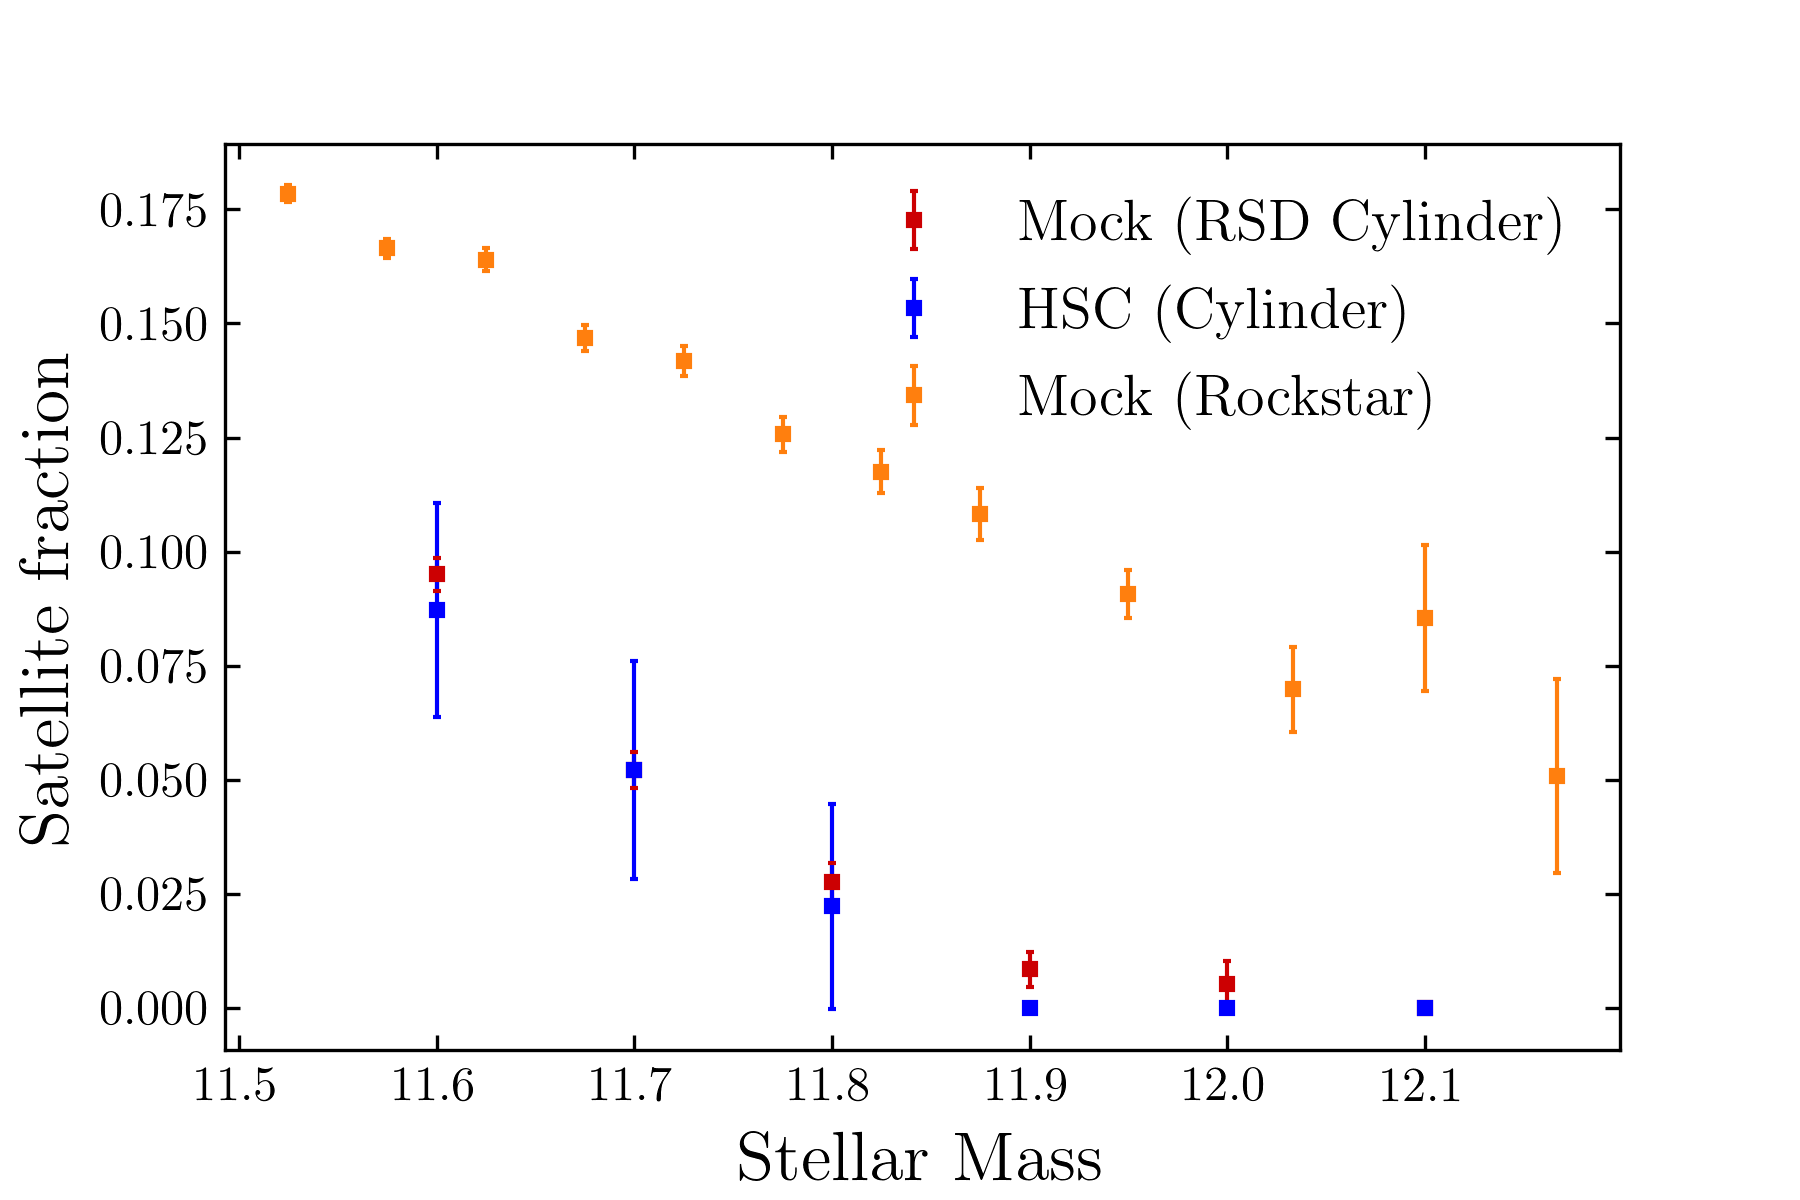
\includegraphics[width=\textwidth]{images/sat_frac.png}
    \caption{Satellite fraction with 2 methods of cluster finding. The first just uses Rockstar cen/sat. The second constructs cylinders 1MPC in radius and 10MPc half length. A galaxy is a satellite if it is in the cylinder of a larger galaxy. The mock matches HSC well.
        I'm not sure how surprised we should be about this as it seems to follow pretty directly from clustering?
    \label{fig:sat_frac}
}
\end{figure}


\subsection{Mag Gap}
Related to the satellite fraction, we can look at the magnitude gap. I'm not really sure whether we can compare to obs because I don't know how we would see this?
\begin{figure}[h]
    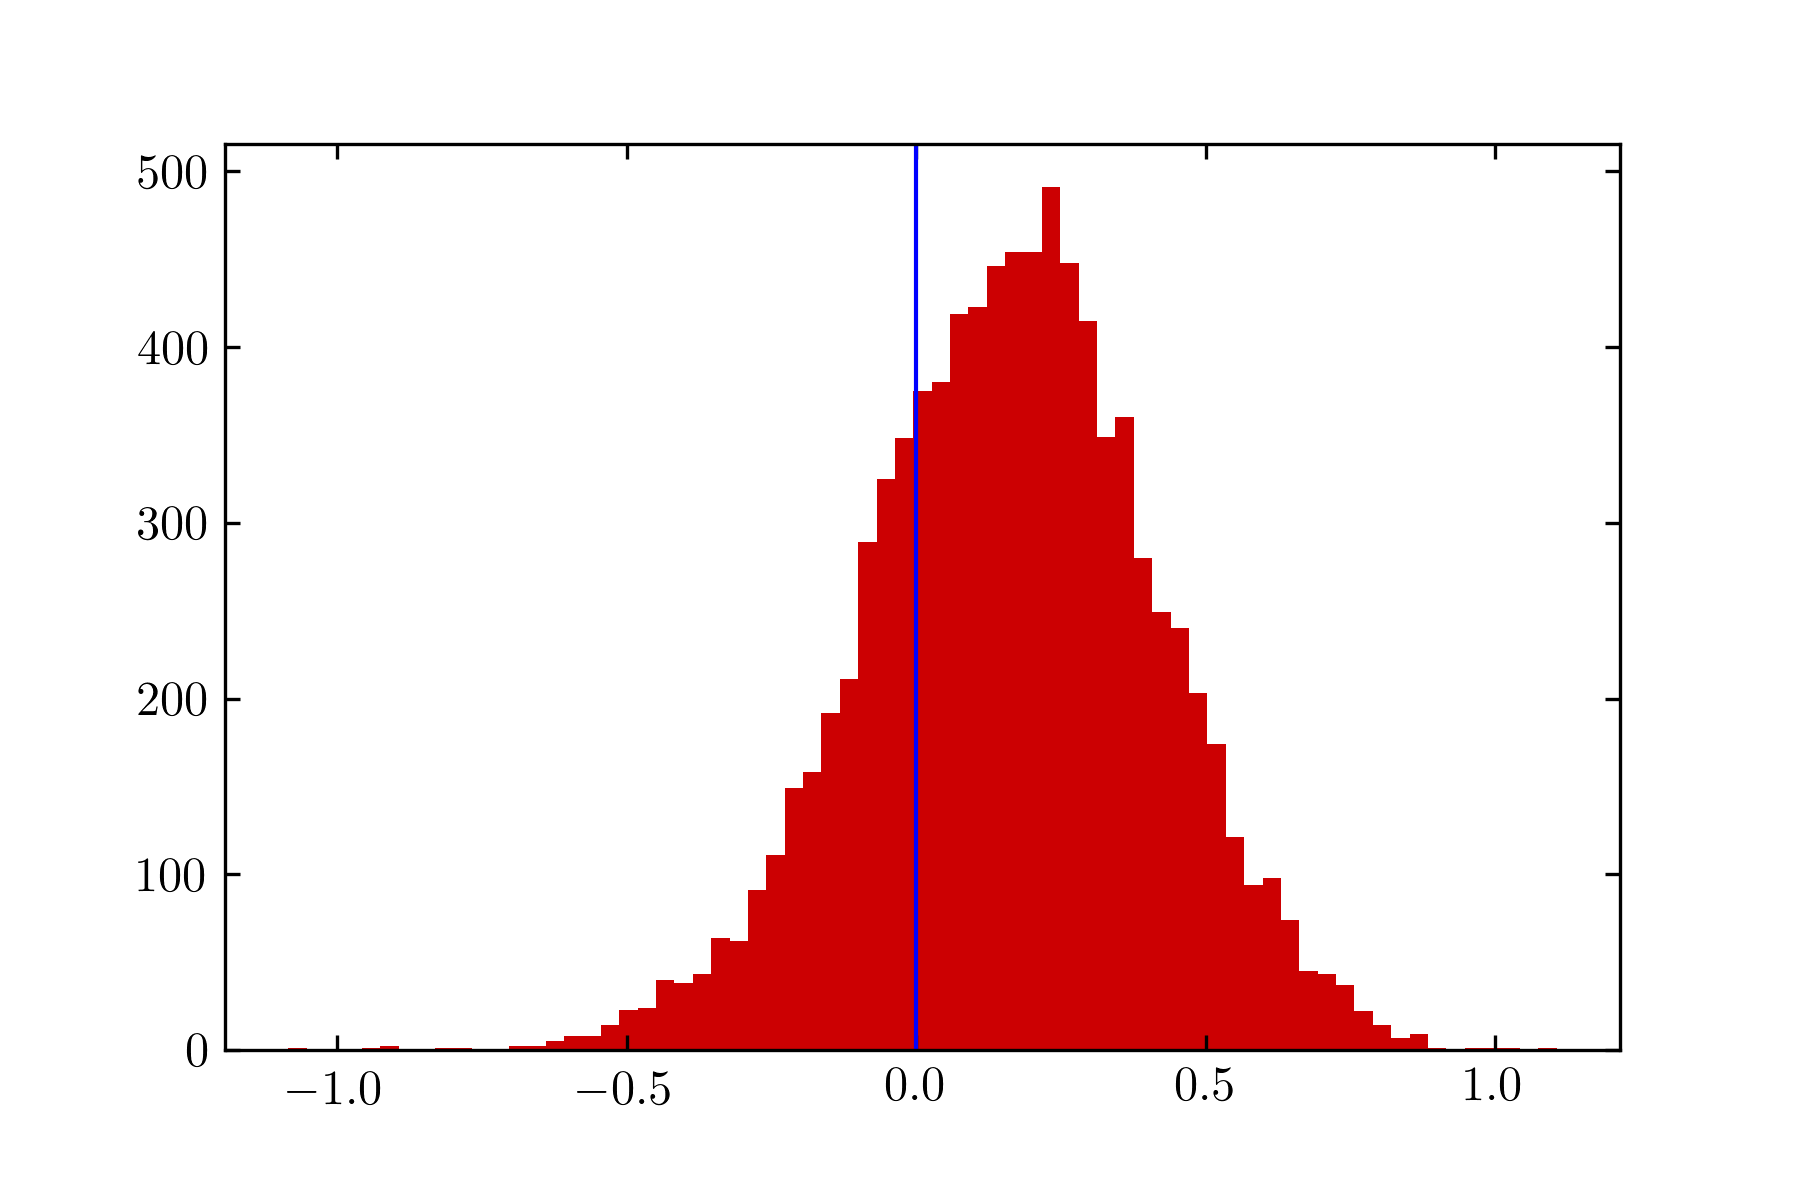
\includegraphics[width=\textwidth]{images/mag_gap1.png}
    \caption{Difference in SM between the central and the largest satellite for halos $>$ 14}
\end{figure}

\begin{figure}[h]
    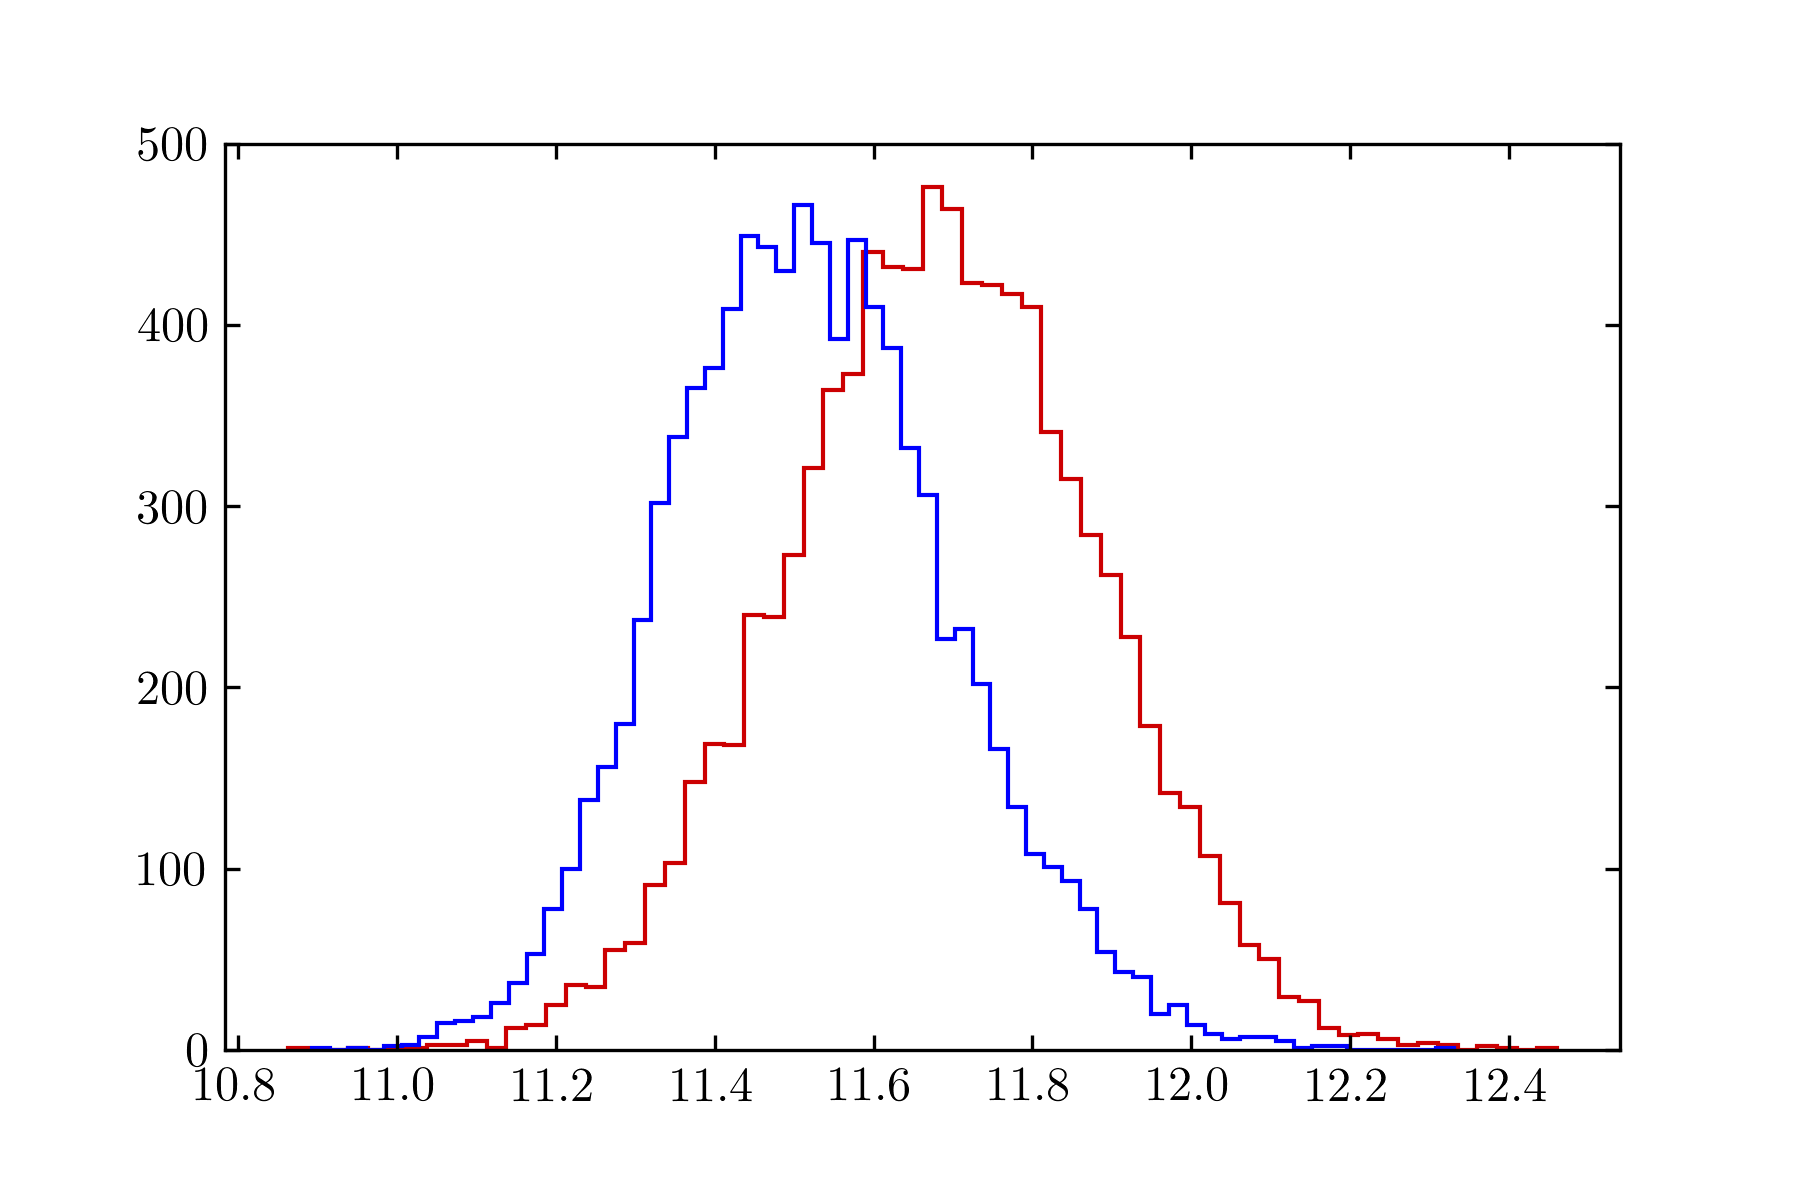
\includegraphics[width=\textwidth]{images/mag_gap2.png}
    \caption{Distribution of SM for centrals and satellites for halos $>$ 14}
\end{figure}

\bibliography{main}
\bibliographystyle{apalike}
\end{document}
